\documentclass{article}

% Run Biber on the file 'journal2'
% Uncomment the following line if you have Biber installed
% !biber journal2

\usepackage{cite} % Add the cite package for citations
% \usepackage[options]{biblatex}
% \addbibresource{part2.BIB}

% Language setting
% Replace `english' with e.g. `spanish' to change the document language
\usepackage[english]{babel}

% Set page size and margins
% Replace `letterpaper' with `a4paper' for UK/EU standard size
\usepackage[letterpaper,top=2cm,bottom=2cm,left=3cm,right=3cm,marginparwidth=1.75cm]{geometry}

% Useful packages
\usepackage{amsmath}
\usepackage{graphicx}
\usepackage[colorlinks=true, allcolors=blue]{hyperref}

\title{Journal2}
\author{Raja Kantheti}

\begin{document}
\maketitle

\section{PART 1}
The browse analysis yielded several valid results, as to how other researchers are tackling the problem. It also gave me a lot of perspective as how the problem evolved and also about the trade-offs that organizations have endured while trying to mitigate this problem. The part of the assignment where I went through journals or conferences gave me an idea of the pace of the current innovation and also determined the novelty factor of my approach towards solving this problem.

\subsection{The three papers I chose:}
\url{https://onlinelibrary.wiley.com/doi/abs/10.1002/cpe.4666}\\
\url{https://www2.eecs.berkeley.edu/Pubs/TechRpts/2017/EECS-2017-157.html}\\
\url{https://dl.acm.org/doi/10.1145/3566053}

\subsection{Rationale of why I chose these three papers:}

I needed a compilation of generic and most used branch prediction techniques used in contemporary Architectures, and I also needed the latest Cores that are being researched to check for compatibility with my approach and also I needed to see the research on mitigations of  side-channel attacks on the target architecture to see how various approaches towards that particular problem can improve my approach. I used the relevant keywords and found many papers to be relevant.

These Three papers gives me the history of Branch Prediction techniques until 2018, Recent Development on the mitigating the SPECTRE attacks which is a known consequence of speculative execution which is a possible result of a Branch Prediction miss and an insight into how modern ISA can be tested against my proposed theory of branch prediction.
% \begin{figure}[h]
% \centering
% 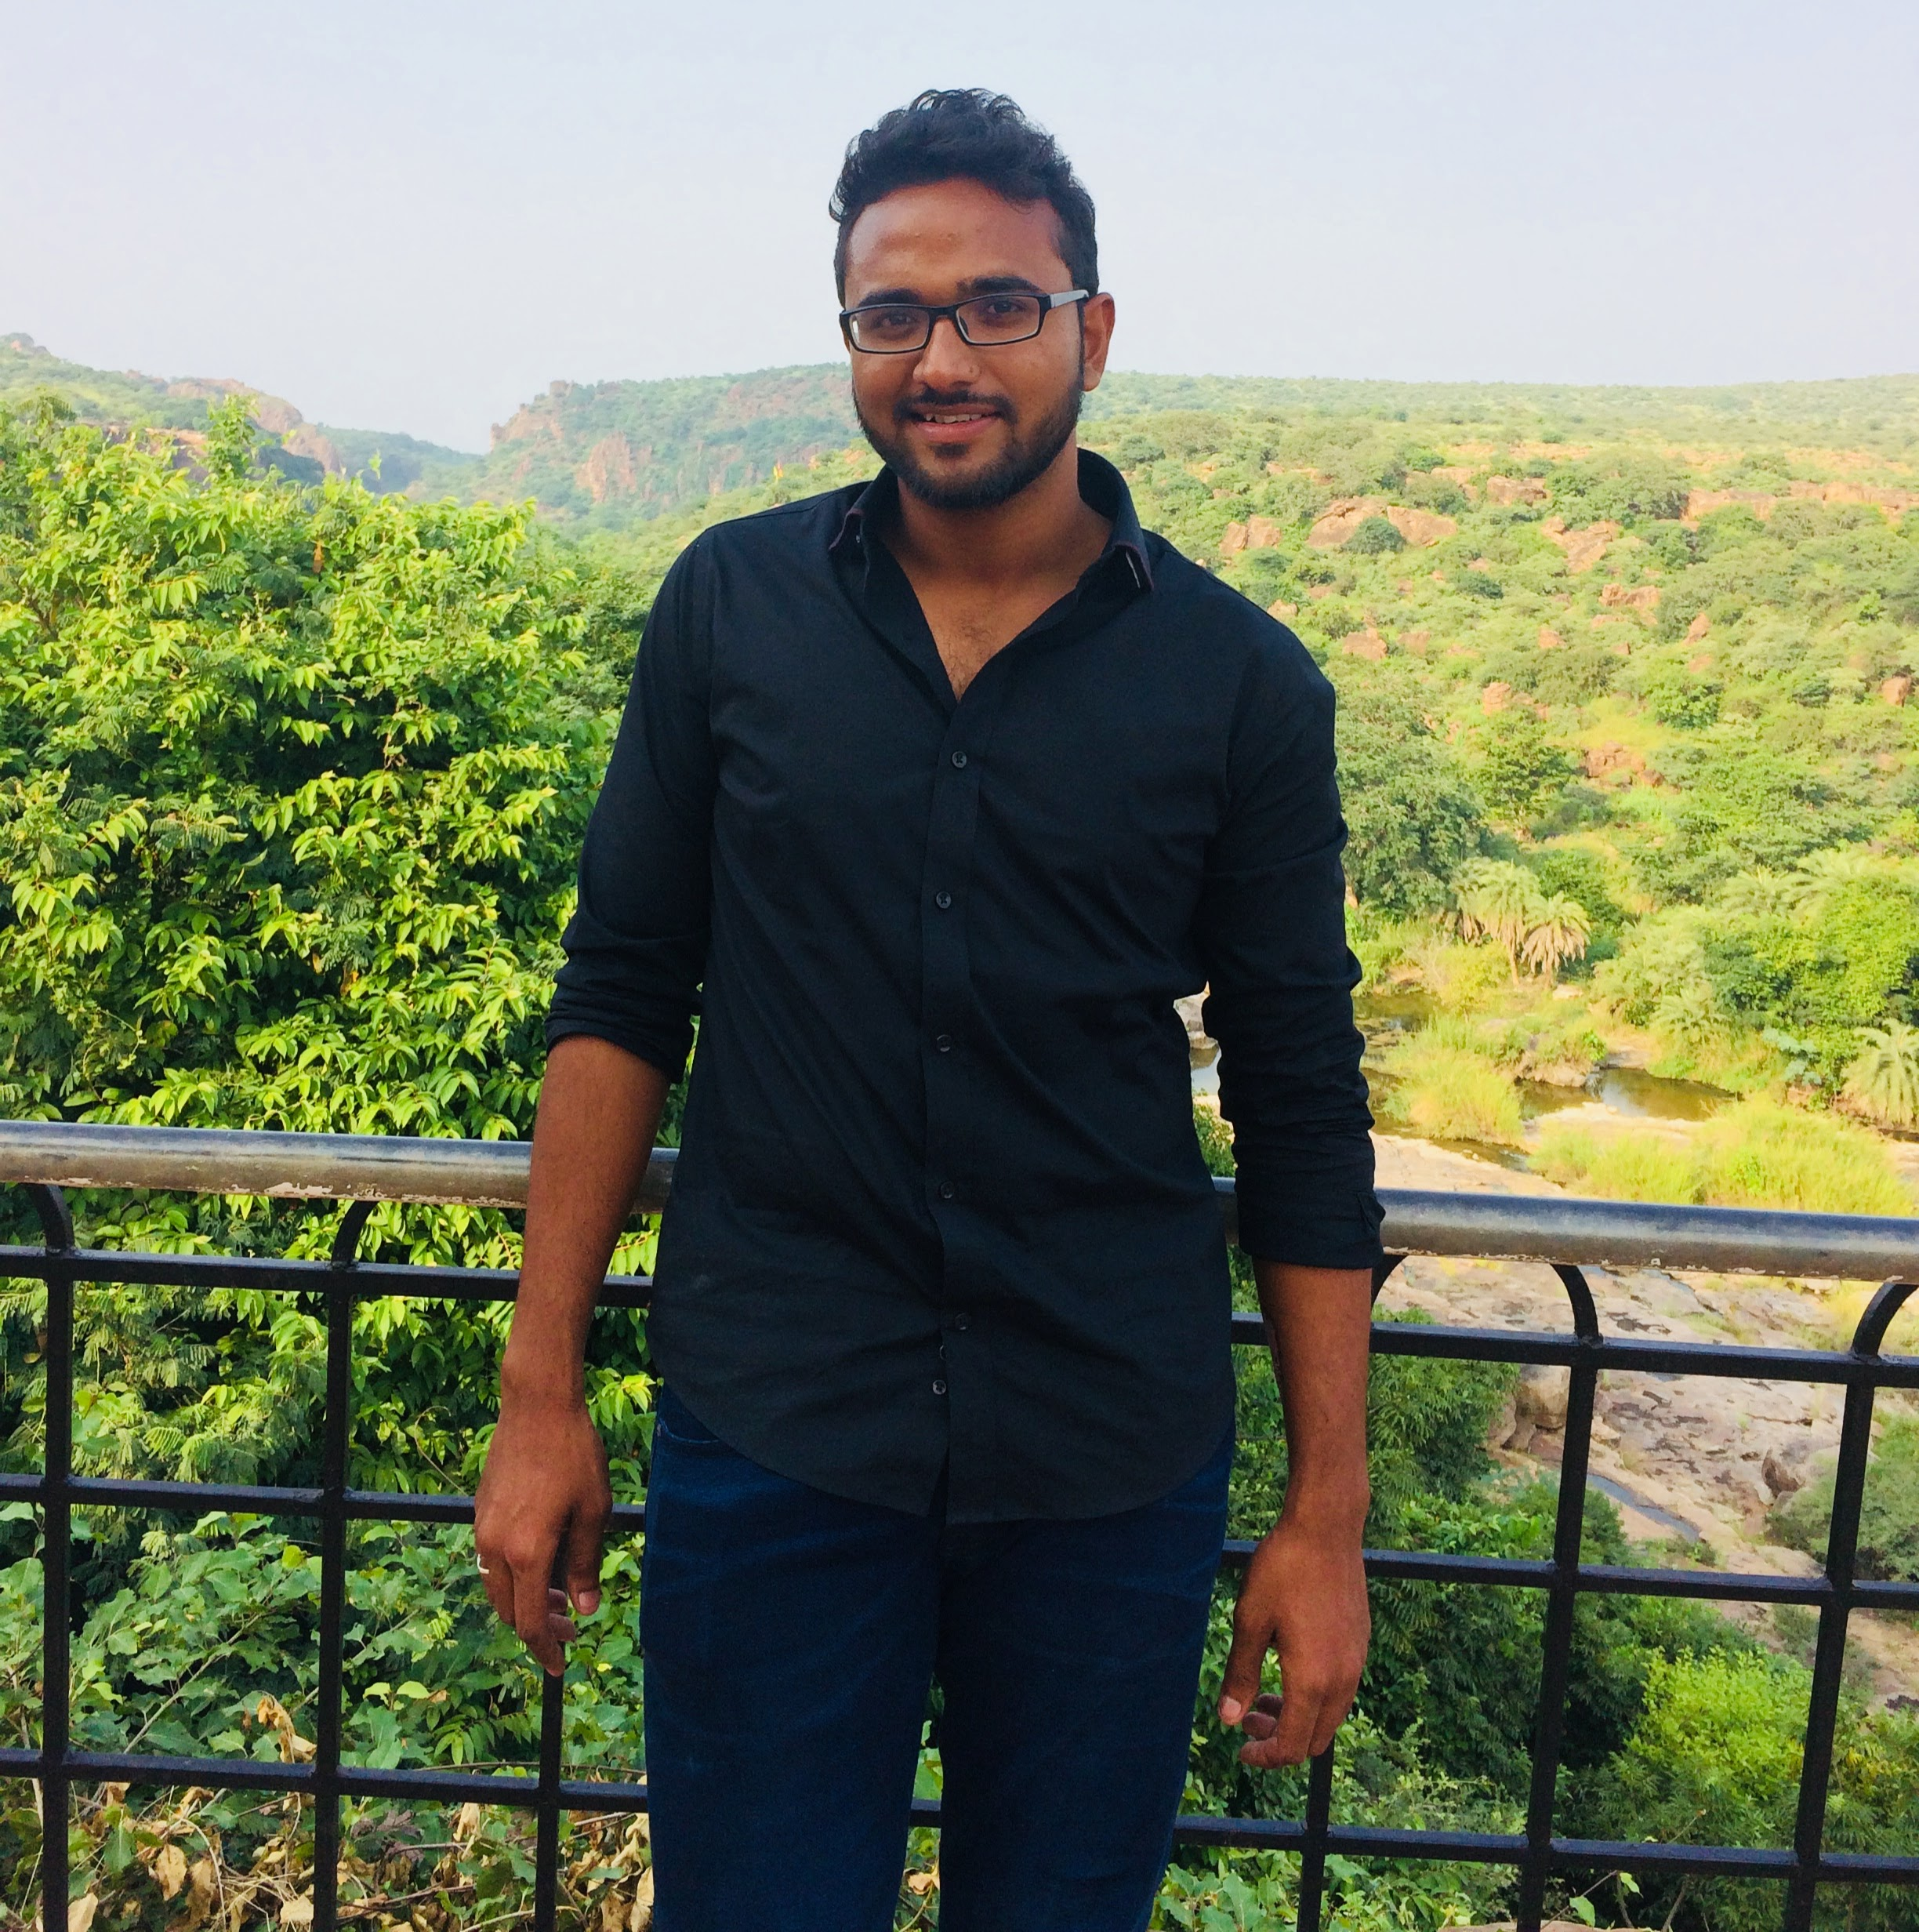
\includegraphics[width=0.25\linewidth]{IMG_1667.JPG}
% \caption{'tis I. }
% \end{figure}
\section{PART 2}
The five papers I skimmed out of the 25 papers are: 

\subsection{Paper 1: }
Survey and Comparison of Pipeline of Some RISC and CISC System Architectures
\paragraph{Notes: }Compares RISC and CISC, 
Super Pipelining: Two-stage super pipelined microprocessor, the task completed by each pipelined segment can be divided into two non overlapping parts and each part can be executed within half a clock cycle.

\subsection{Paper 2:}
The optimum pipeline depth for a microprocessor
\paragraph{Notes: }Old Paper, 
Used a proprietary simulation system to simulate various versions of Pipeline for varying depths. tested mainly for SPEC benchmark suite. Need to study the section titled “Theory” more.
Not really sure about how the methodology can relate to the modern workloads.

\subsection{Paper 3:}
Dynamic branch prediction for a VLIW processor
\paragraph{Notes: }Selective Branch Prediction for VLIW Processors. mixinf predicted and delayed branches yielded performance improvements.

\subsection{Paper 4:}
Reducing the branch penalty in pipelined processors
\paragraph{Notes: }"Branch bypass and multiple prefetch”  this is what you are thinking along with multiple decode units. Read more about this as this contains some methods to quantify such hypothetical machines.

\subsection{paper 5:}
Branch Prediction — RISCV-BOOM documentation
\paragraph{Notes: }Clear explanation aboout the BOOM Outof order RISCV core with emphasis on it’s branch prediction strategy.

The Remaining 21 Papers are Group Cited \emph{here}\cite{augustusk.uhtDisjointEagerExecution2002,balasubramanianNoPenaltyControlHazard2024,BranchPredictionUnit,calderFastAccurateInstruction1994,emmaCharacterizationBranchData1987,eversUsingHybridBranch1996,evtyushkinBranchScopeNewSideChannel2018,hartsteinOptimumPipelineDepth2002,heSurveyComparisonPipeline2023,johnsonBranchPredicationUsing1992,kocherSpectreAttacksExploiting2020,koruyehSpectreReturnsSpeculation2018,kostromitinAnalysisMostCommon2020,liConditionalSpeculationEffective2019,linBranchPredictionNot2019,maisuradzeSpeculoseAnalyzingSecurity2018,mohammadiDemandDynamicBranch2015,StaticMethodsHybrid,vitekValidatingSideChannel,wallSpeculativeExecutionInstructionLevel,zhangHybridBranchPrediction2002}

\section{PART 3}
\subsection{Table of Contents}
\paragraph{ACM Transactions on Architecture and Code Optimization\ref{fig:Table of Contents}}
\begin{figure}[ht]
    \centering
    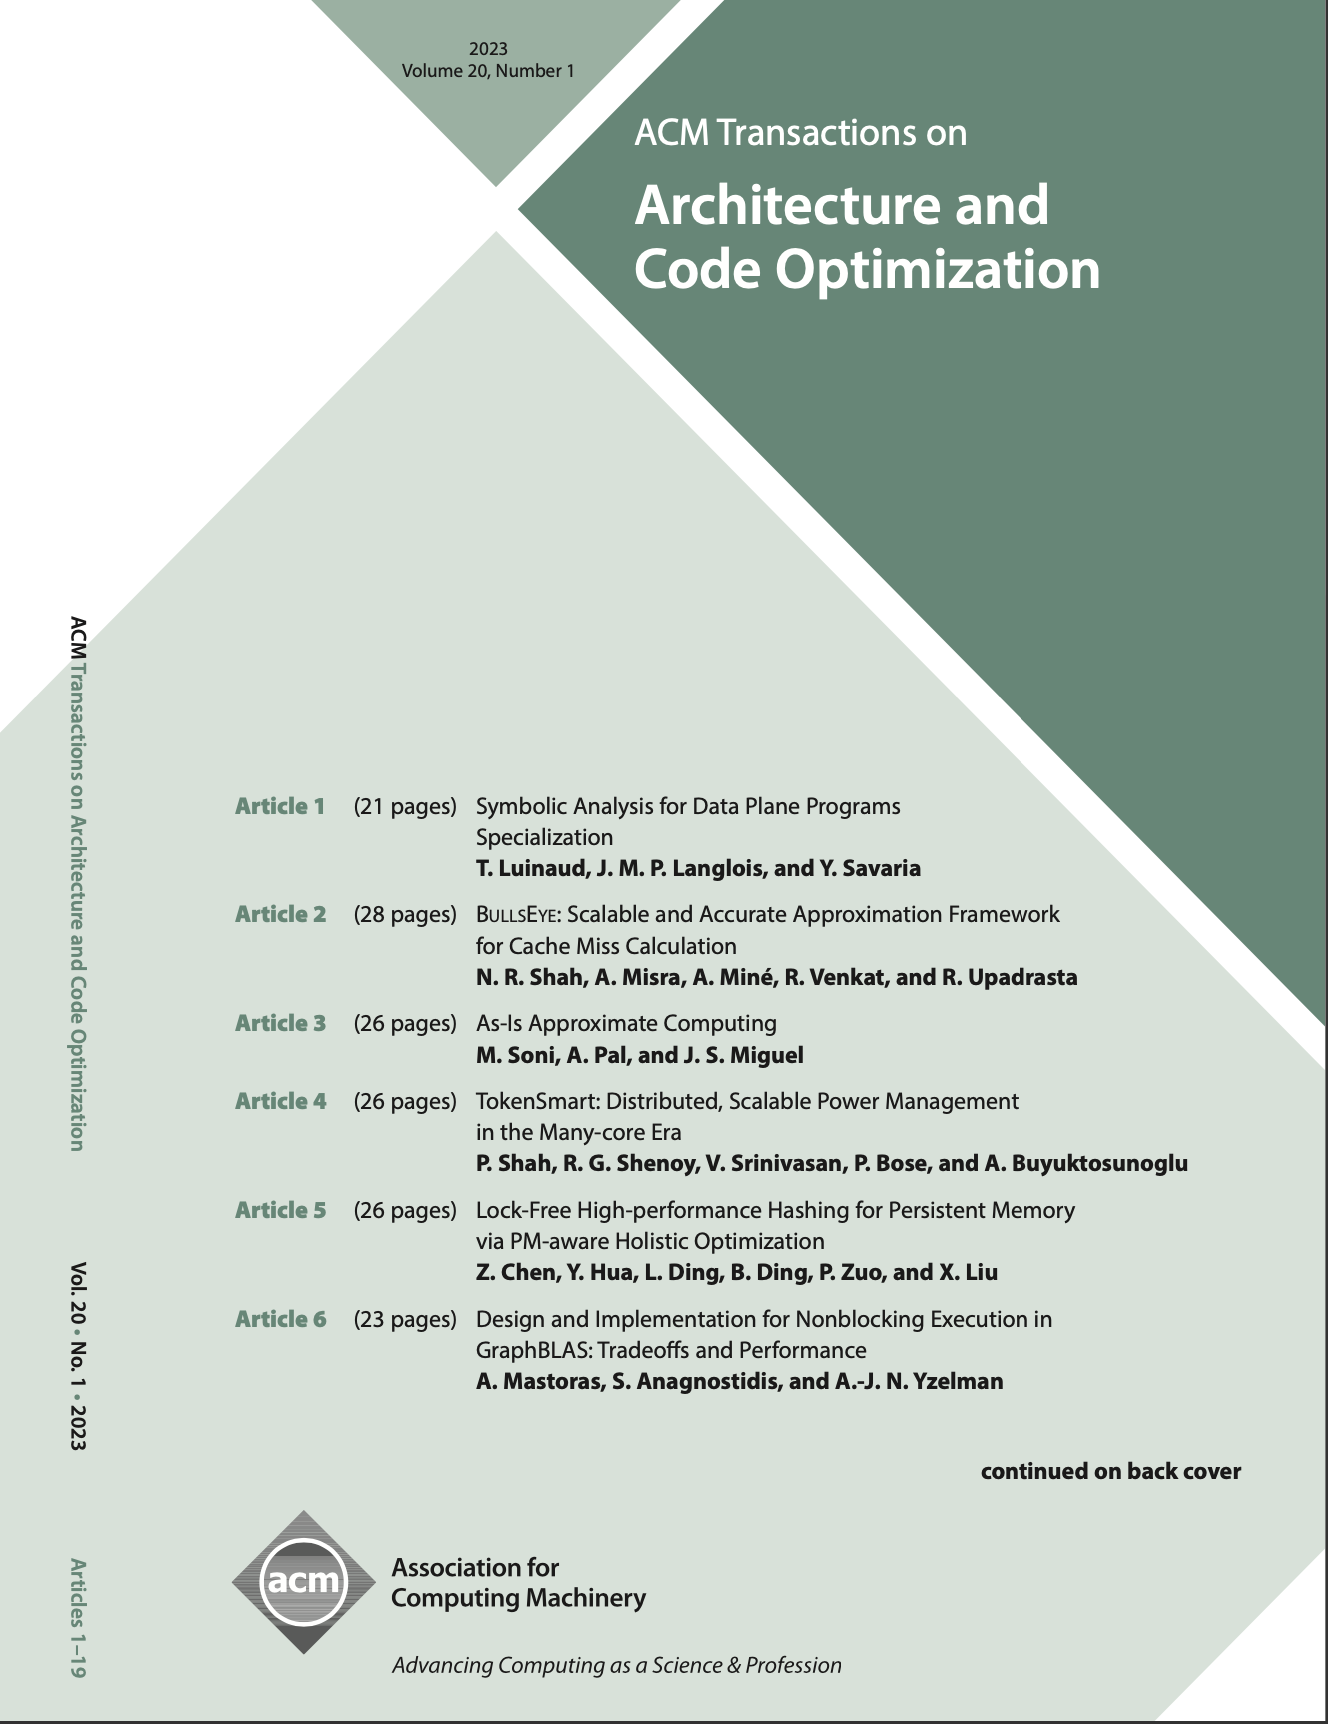
\includegraphics[width=0.25\linewidth]{1.png}
    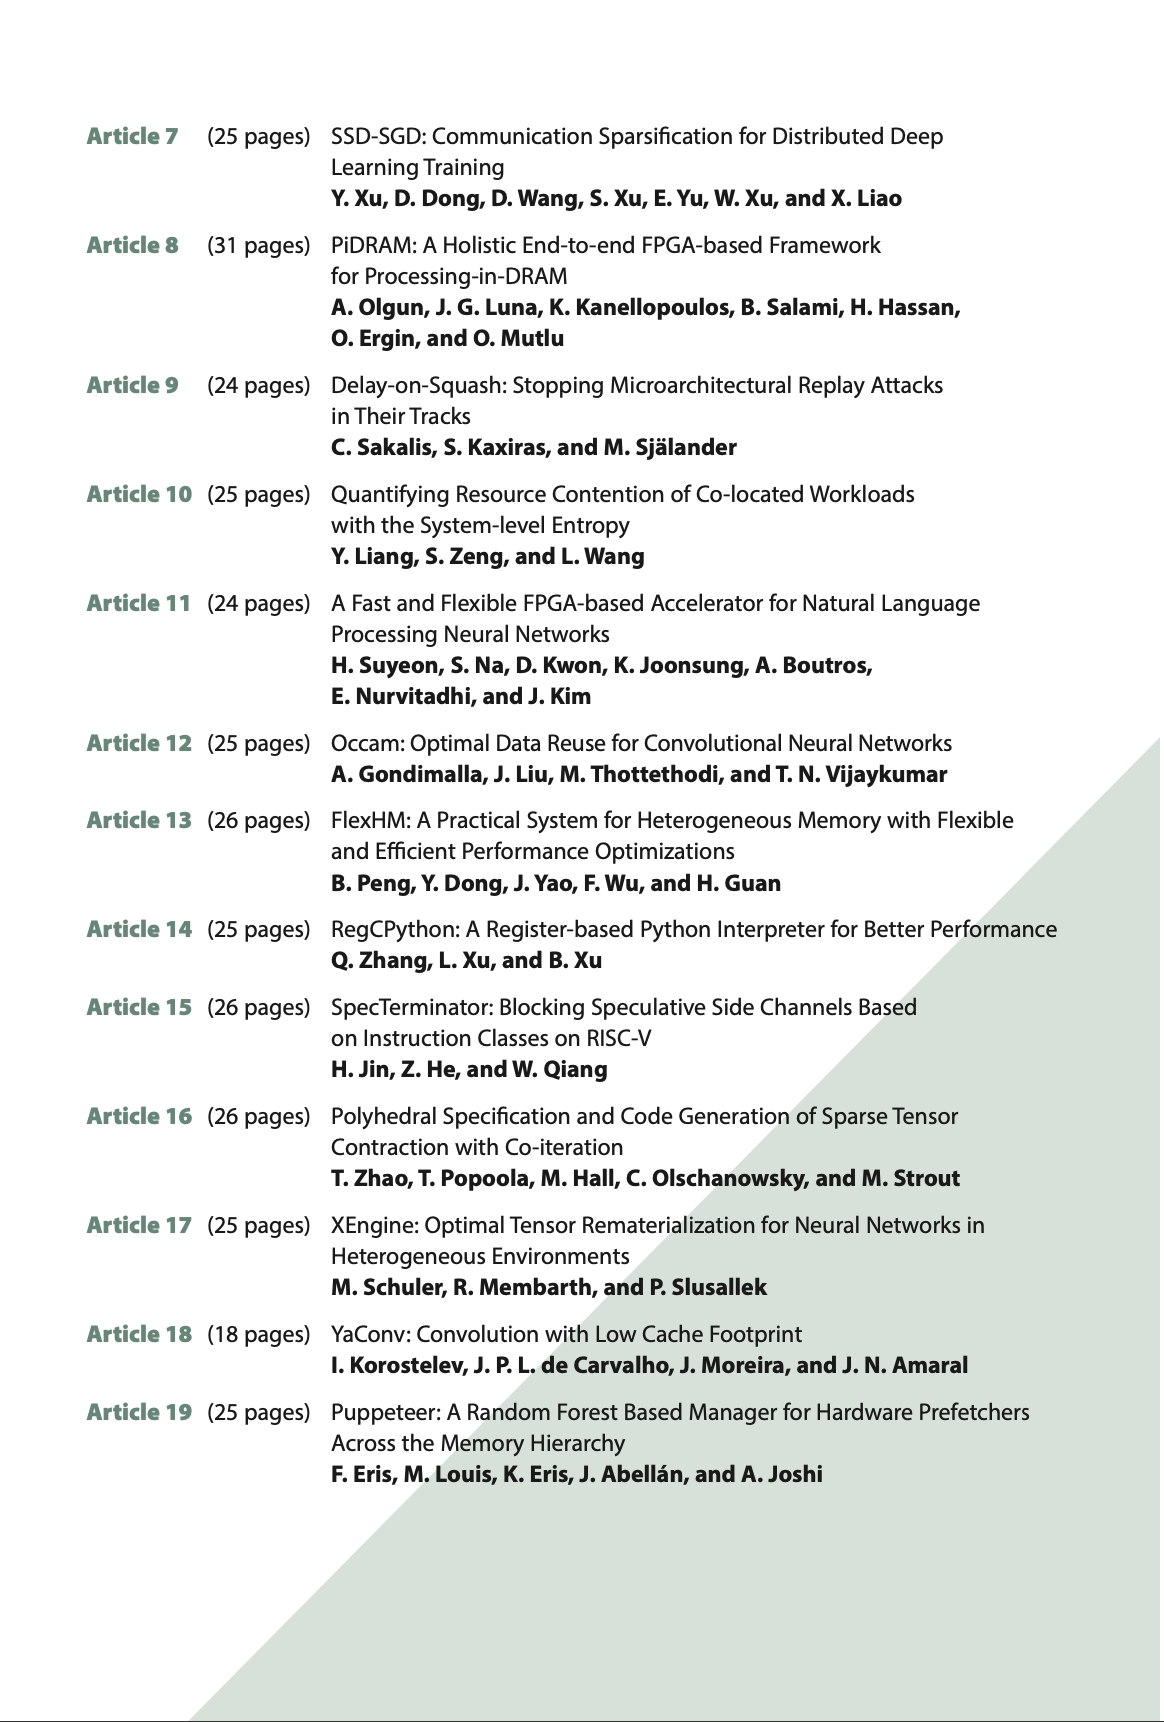
\includegraphics[width=0.25\linewidth]{2.png}
    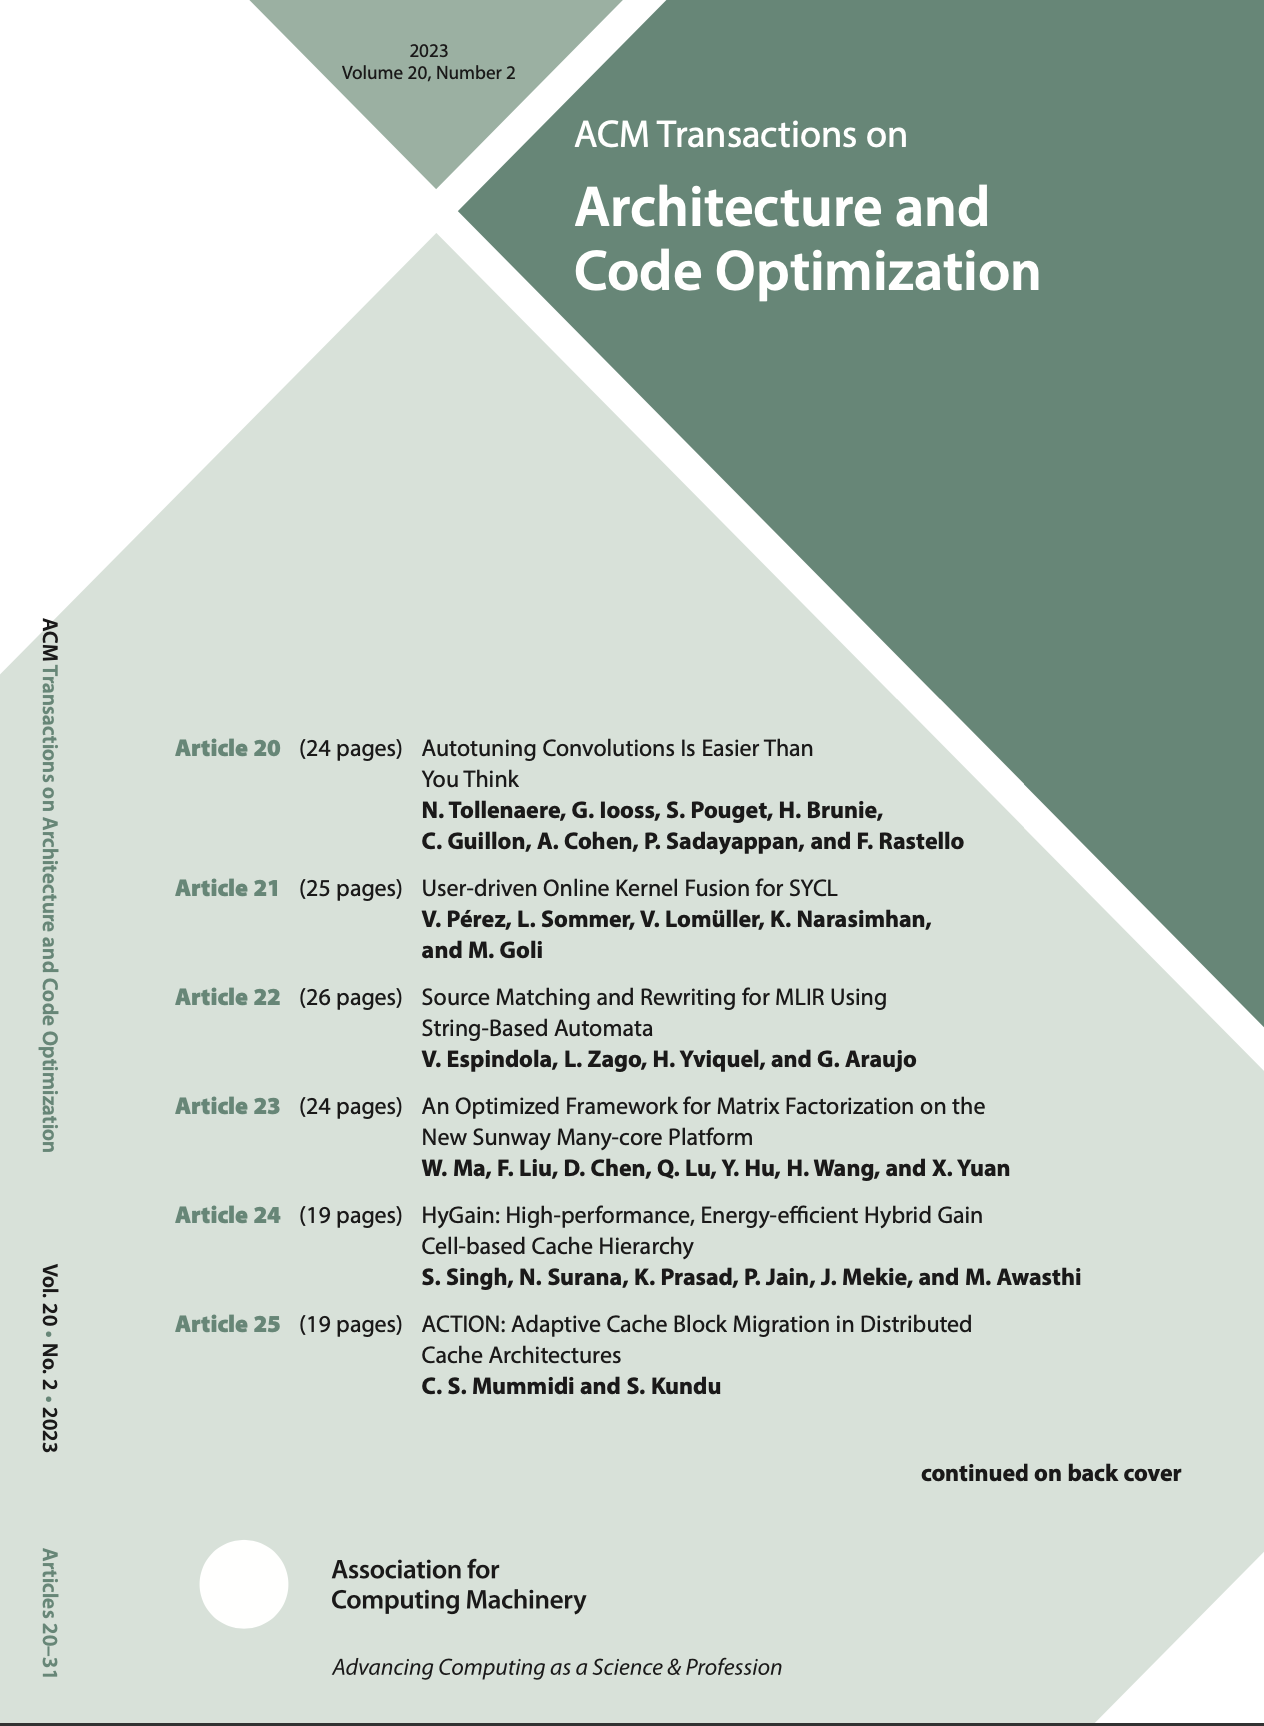
\includegraphics[width=0.25\linewidth]{3.png}
    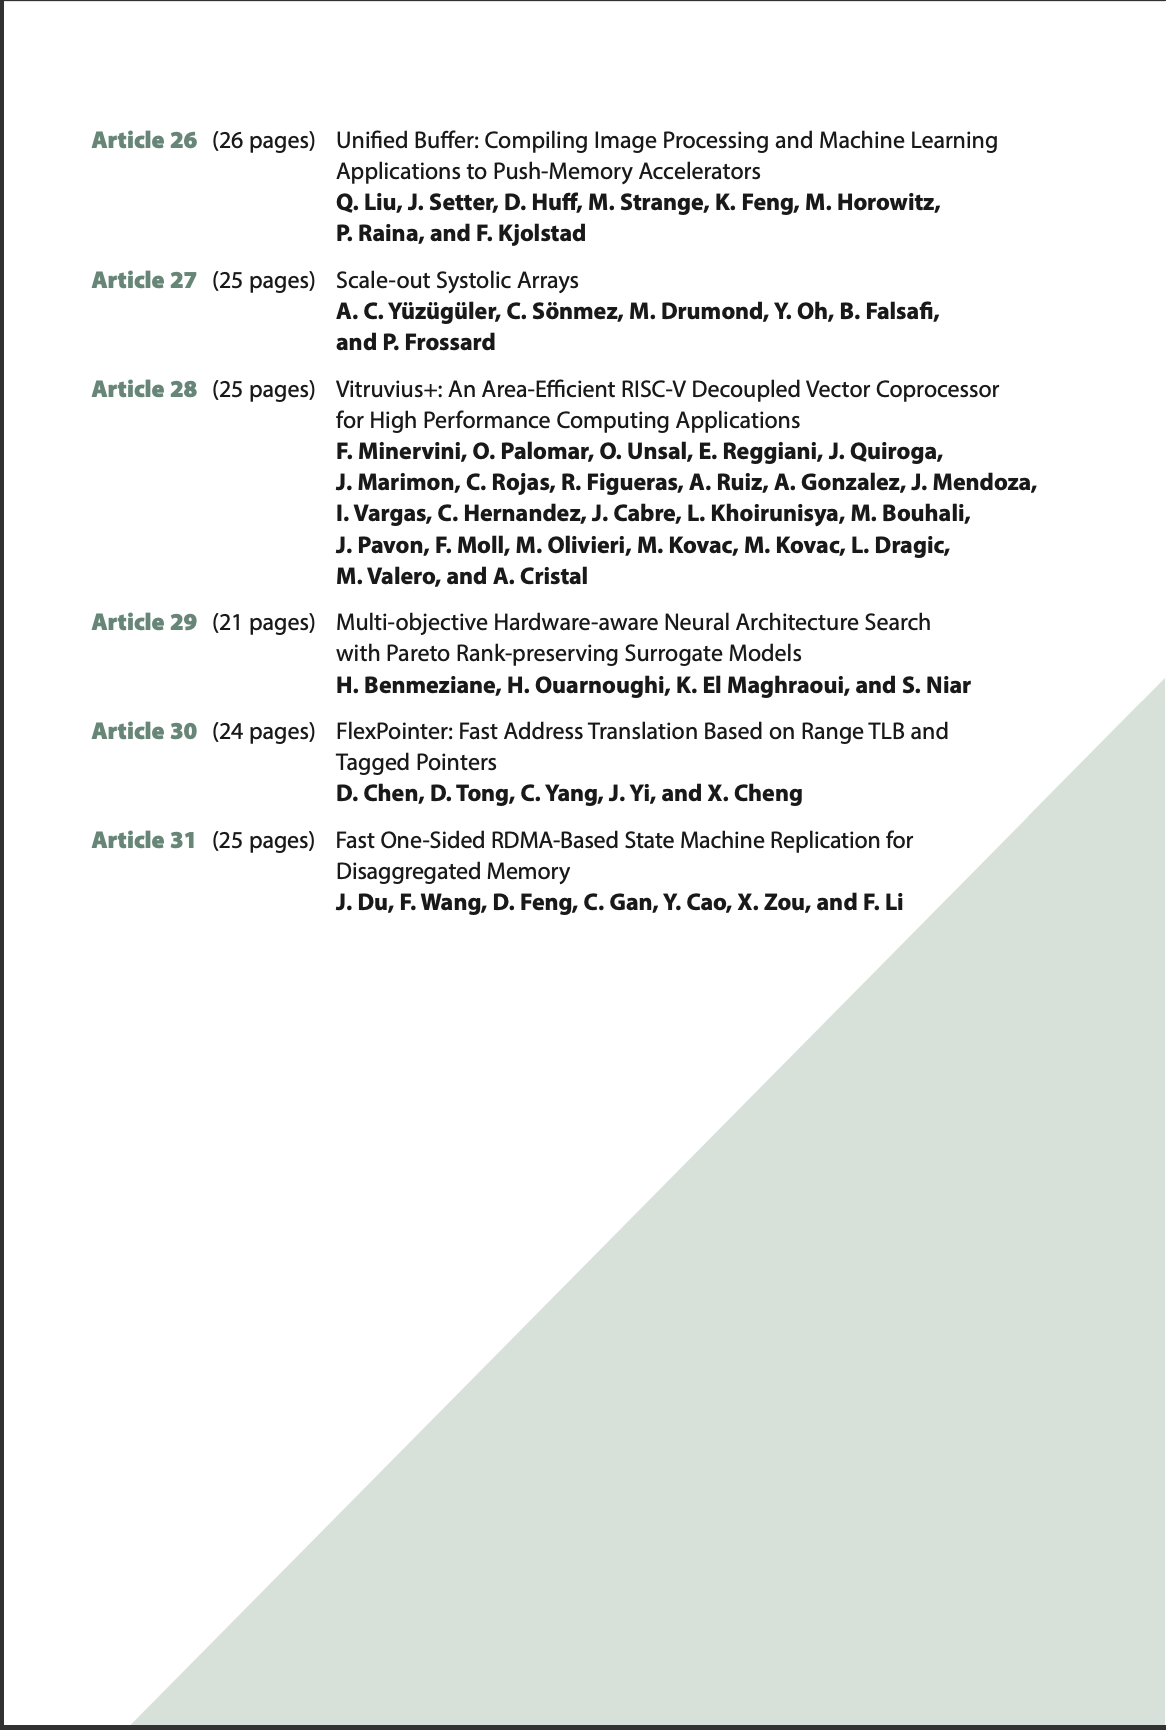
\includegraphics[width=0.25\linewidth]{4.png}
    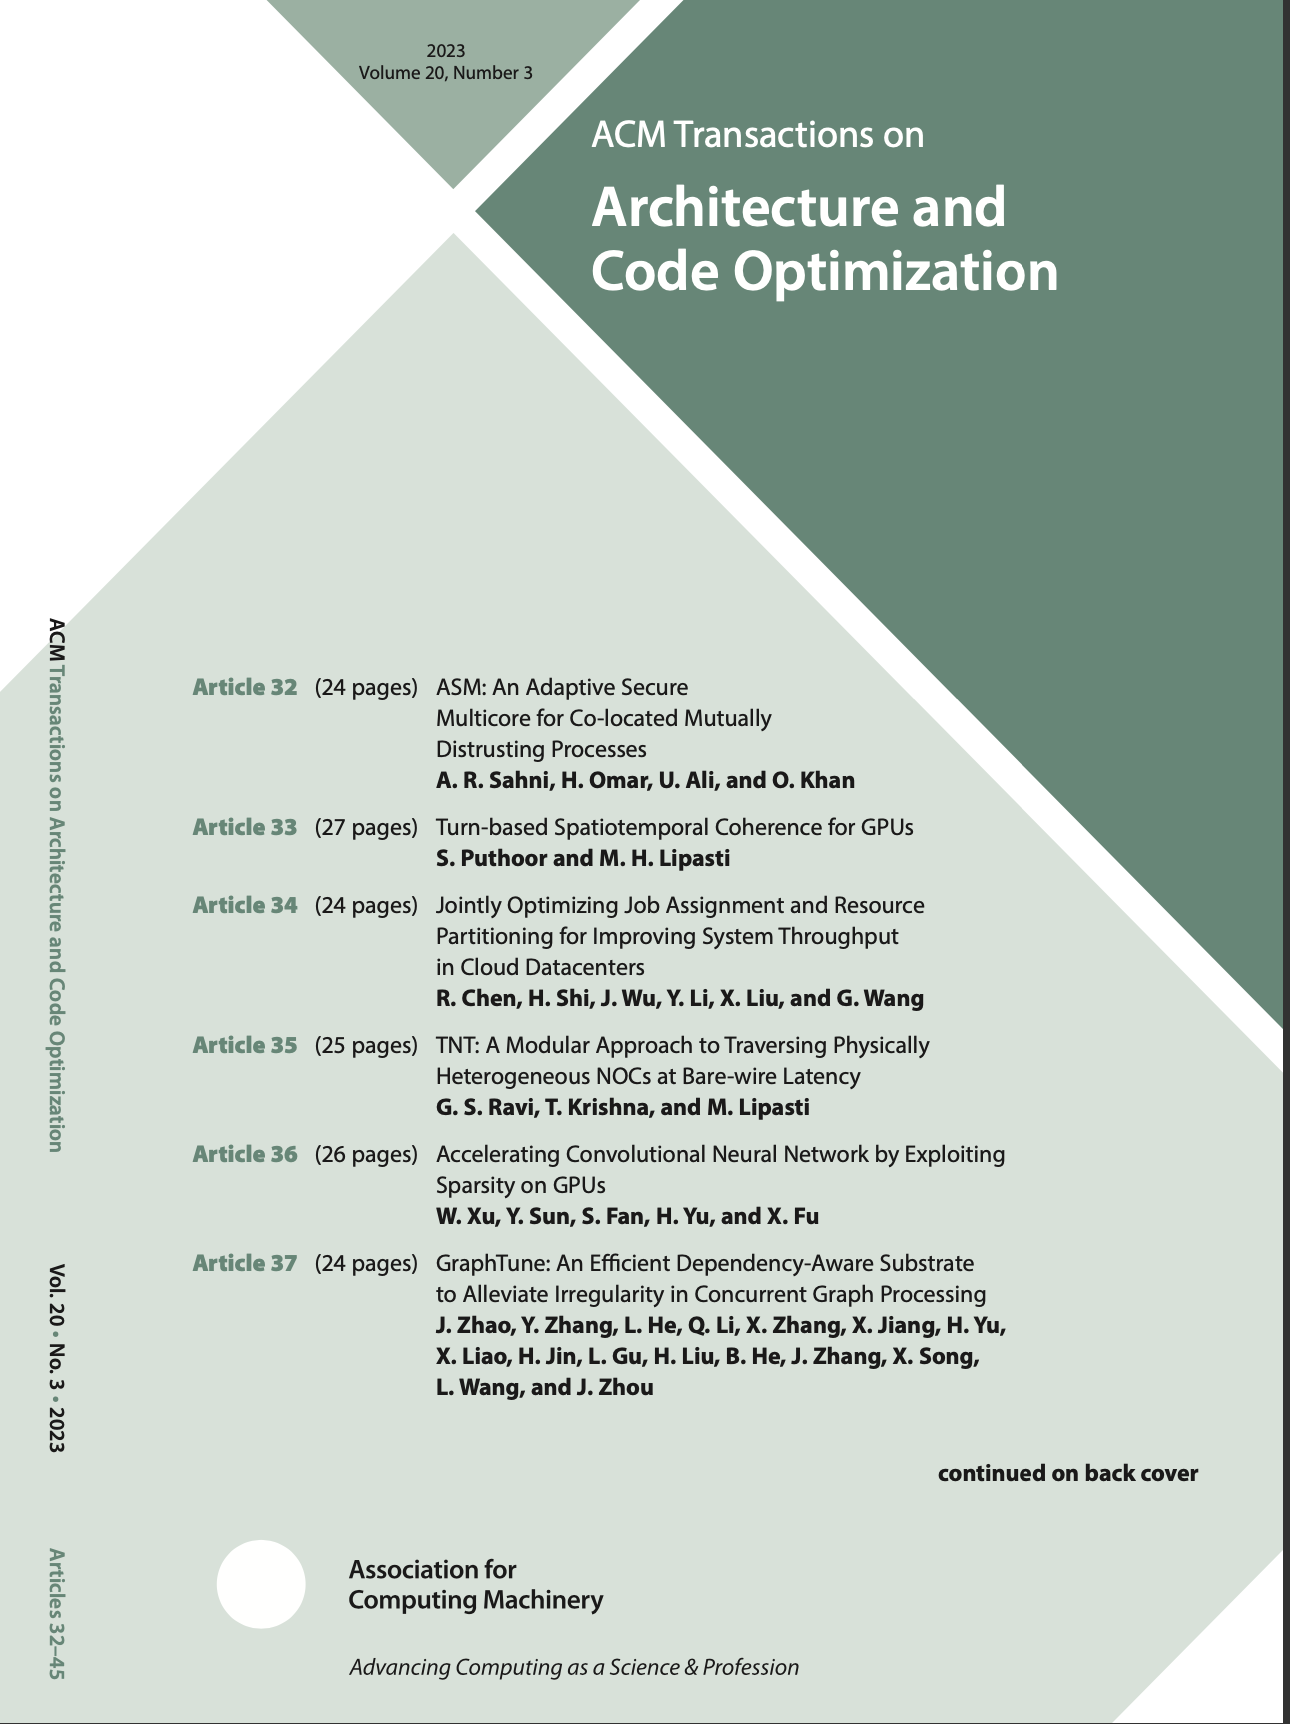
\includegraphics[width=0.25\linewidth]{5.png}
    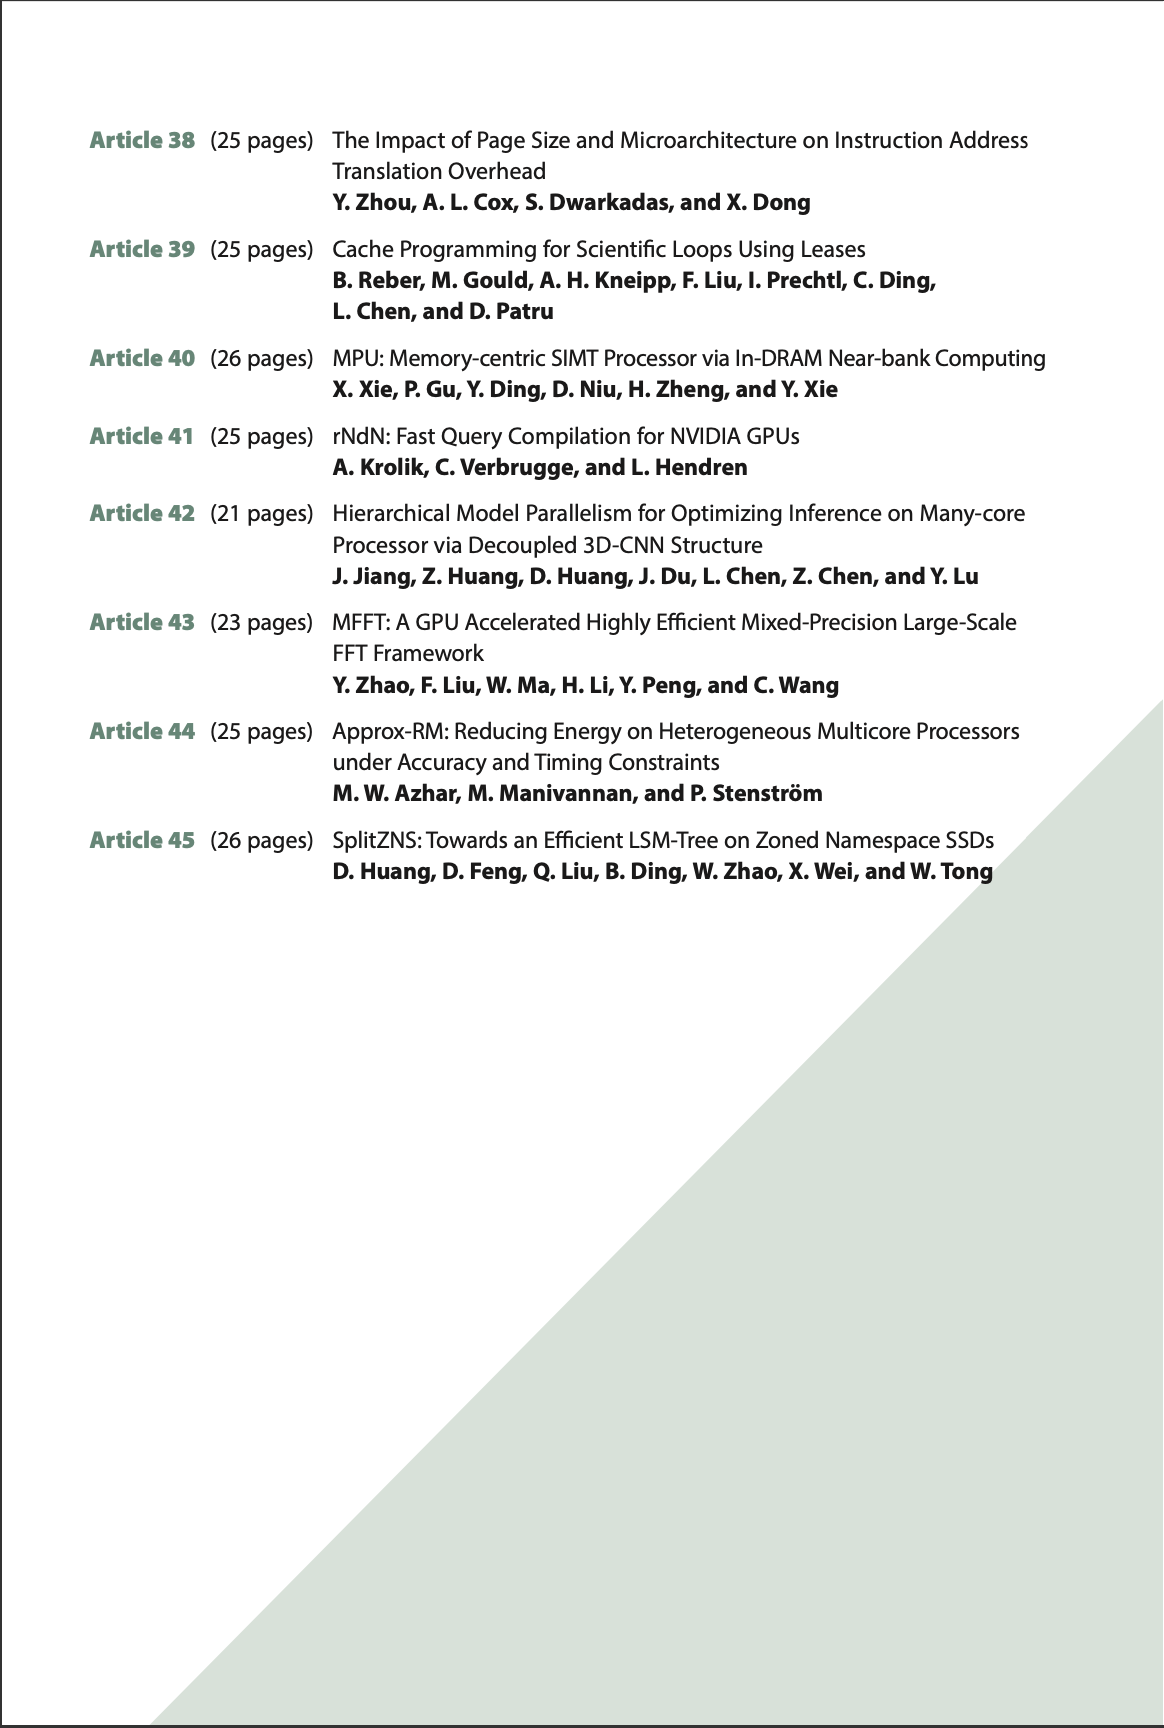
\includegraphics[width=0.25\linewidth]{6.png}
    \caption{Table of Contents. }
    \label{fig:Table of Contents}
\end{figure}
\paragraph{Why I chose this Journal:} I chose ACM TACO as the journal because of its diversity in topics and specialized focus on subjects like parallel computing, pipeline optimizations, Computer Architecture, etc. 
\subsection{My Learning process: }
Browsing, Skimming, and Scanning of the research papers were very productive and liberating. The time elapsed between starting and ending the assignment was the most I had ever done since I thought of my thesis problem. The process of searching for papers and journals, which gave me more insight into what was happening in the field, gave me a broader perspective on my approach to solving the problem. 

Although it was a tedious task at the beginning of the assignment, I got into flow in part two when I started skimming the 5 papers. I learned how to search papers and what to look for when trying to find relevance to my research. I saw how much I could expand my research to solve other problems and find new evaluation methods if I ever got results. I also understood how I could better express my research to my advisor.
\subsection{Raw notes from critical reading three papers: }
\paragraph{Paper 1: Delay-on-Squash: Stopping Microarchitectural Replay Attacks in Their Tracks}
\subparagraph{Notes: }Critical REad, 45 sec, Scan it, Talks about halting/disallowing speculative execution after page miss, very closely related to your work.The poinnt is not to significantly impact the performance but to stop replay attacks by tracking the squashes. Bloom filters are suedd to deteect if a PC is ina set after hashing it if yes, then a bulk reset is the only way to reset the filter which will change the pc. approach is to ise two bloom fileters and switch between them. at ny point in time only fileter is tagged as active. the other one will wait to be cleard. after the the active filter is cleared the status is altered on both filters. take figure 4 for IPC metric.
\paragraph{Paper 2: SpecTerminator: Blocking Speculative Side Channels Based on Instruction Classes on RISC-V}
\subparagraph{Notes:}Critical READ,45 seec, scan it, talks about bblocking SPECTRE attacks in RISCV. Need to get the grip on different types of SPECTRE attacks. You may actually be mitigating only one based on the text. Delayed execution strategies, TLB request ignoring, Classifiation of LOAD instructions in ISA whic are speculative depended baased on the architectural changes., TAble 1 has existing hardware defecnecs against spectre attacks, need to critically read those in hte coming days. Experimental setup is unique instead of using genric simiulation like gem5 using FPGA simulation platform will give more access towards the architectural changes ? this doesn’t mean it is biased, it is required for the analysis of the experiment results. I donno BOOM might not have been the best processor to choose, a multiple issue inorder may be would’ve yielded different results ? Finally, SPECTerminator has a lowe performance ocverheard than other hardwaare or OS based techniques.
\paragraph{Paper 3: The Impact of Page Size and Microarchitecture on Instruction Address Translation Overhead}
\subparagraph{Notes: }Critical rEad, 2:00, Scan it, Talks about how page size and pipeline can impact hardware overhead of address translation. Quatification of different TLB organization based on overhead. TLB overhead is about 13.44% of execution cycles. taken experimental setups XEon and Ryzen Free BSD OS. table 1 for TLB structures. Fig 1 for comparisions with differnt workloads.
\nocite{*}
\bibliographystyle{unsrt}
\bibliography{part2,Part3}
% \bibliography{Part3}
\end{document}